\documentclass[11pt]{article}
\usepackage{latexsym}
\usepackage{amsmath}
\usepackage{amssymb}
\usepackage{amsthm}
\usepackage{epsfig}
\usepackage[tight]{subfigure}

\usepackage{amsmath}

\DeclareMathOperator*{\minimize}{min}
\DeclareMathOperator*{\maximize}{max}

\usepackage{algorithm}
 %on linux you may need to run sudo apt-get install texlive-full to install algorithm.sys
\usepackage{algorithmic}

\usepackage{verbatim}

\newcommand{\handout}[5]{
  \noindent
  \begin{center}
  \framebox{
    \vbox{
      \hbox to 5.78in { {#1} \hfill #2 }
      \vspace{4mm}
      \hbox to 5.78in { {\Large \hfill #5  \hfill} }
      \vspace{2mm}
      \hbox to 5.78in { {\em #3 \hfill #4} }
    }
  }
  \end{center}
  \vspace*{4mm}
}

\newcommand{\lecture}[5]{\handout{#1}{#2}{#3}{#4}{#5}}
\newcommand{\collision}[0]{\mathrm{collision}}
\newcommand{\nocollision}[0]{\overline{\collision}}

\newcommand*{\QED}{\hfill\ensuremath{\square}}

\newtheorem{theorem}{Theorem}
\newtheorem{corollary}[theorem]{Corollary}
\newtheorem{lemma}[theorem]{Lemma}
\newtheorem{observation}[theorem]{Observation}
\newtheorem{proposition}[theorem]{Proposition}
\newtheorem{definition}[theorem]{Definition}
\newtheorem{claim}[theorem]{Claim}
\newtheorem{fact}[theorem]{Fact}
\newtheorem{assumption}[theorem]{Assumption}
\newtheorem{note}[theorem]{Note}

% 1-inch margins, from fullpage.sty by H.Partl, Version 2, Dec. 15, 1988.
\topmargin 0pt
\advance \topmargin by -\headheight
\advance \topmargin by -\headsep
\textheight 8.9in
\oddsidemargin 0pt
\evensidemargin \oddsidemargin
\marginparwidth 0.5in
\textwidth 6.5in

\parindent 0in
\parskip 1.5ex
%\renewcommand{\baselinestretch}{1.25}

\begin{document}

\lecture{Statistical Techniques in Robotics (16-831, S22)}{Lecture \#22
  (Monday, April 11)}{Lecturer: Kris Kitani}{Scribes: Jonathan Schwartz, Husam Wadi}{Imitation Learning \& LP-IRL}

%RL SECTION REQUIRES AT LEAST 1 CITATION
\section{Review}
In the previous lectures, we went over Reinforcement Learning (RL) and had explored several types of RL:

\begin{enumerate}
    \item Policy-based
    \item Hybrid
    \item Value-based
\end{enumerate}

We then explored these topics in depth and how each approach has subsets, such as Model-based and Model-free, and within these subsets there are various approaches such as Monte Carlo, Actor-Critic, Policy Gradient, N-step TD learning, and the list goes on. In this lecture, we switch over to Imitation Learning (IL) and explore from a top-down high-level perspective what IL addresses. We will also delve into what Inverse Reinforcement Learning (IRL) is and how it is used in the context of IL. The advantages IL has over RL is that instead of creating and penalizing specific rewards, such as joint toques and motor speeds, which may be difficult to design around, IL instead rewards based on imitating a whole subset of actions. This is advantageous because IL simplifies the setup and training procedure for complex tasks like robot grasping, where it is not clear what specific value should be the reward function. It also makes systems with large state spaces feasible, as with traditional RL it is costly to train specific rewards across massive tensors.  

%This section serves as a review of the previous lecture and any other context required to frame the content of the current lecture. 

%You may format the scribes in any way you like, aside from changing font style, size and page format. Please use subsections and paragraphs to increase the readability of your notes.

%Length requirement 1-2 pages.
        
\subsection{Reinforcement Learning: Markov Decision Process}

RL is an algorithmic approach described as an agent learning (or closely approximating) an optimal policy that maximizes a reward function. RL problems are often modeled as grid based Markov Decision Processes (MDP) that allows us to use powerful equations such as the Bellman Equation: An equation which defines an inductive/recursive relationship between value functions and constraint optimizations. To setup a MDP we can define the problem with $(S, A, P, r, H, \rho)$, where $S$ is equal to the state, $A$ is equal to the action, $P$ is the transition dynamics, $P(s'|s,a)$ is equal to the probability of achieving $s'$ from state $s$ through action $a$, $r$ is equal to the reward, $H$ is equal to the planning horizon, and $\rho$ is equal to the probability distribution of the initial state $S$. 

$\pi(a|s)$ is the probability that action $a$ takes place at state $s$. Starting from the initial state, a trajectory routes the path from that state to the planning horizion defined by this relationship: $\tau=\{s_1,a_1,s_2,...,s_H,a_H,s_{H+1}\}$ given $s_1\sim \rho$, $a_t\sim \pi(\cdot|s_t)$ and $s_{t+1}\sim \pi(\cdot|s_t, a_t)$. Through this MDP setup, an RL algorithim finds the optimal policy that maximizes the reward: $R(\tau) = \sum_tr(s_t,a_t)$.


\subsection{Reinforcement Learning: Value vs Policy Function}

To delve into the difference between Value vs Policy Functions, let us review the three main archetypes of RL in detail:

\begin{itemize}
    \item \textbf{Policy-based}: Back deriving reward optimization directly through reward interactions with the environment, without an explicit value function.
    \item \textbf{Hybrid}: A mix of Policy-based and Value-based approaches.
    \item \textbf{Value-based}: Through interactions with the environment, we define a value function that scores the outcome of state $s$ and action $a$ to $s'$ and the reward $r$ that is achieved through this interaction. This value function is used to improve the policy which then increases the reward output.
\end{itemize}

The issue with these approaches is that we have no prior to use, so we must use stochastic and predictive methods to explore the state space. This may take quite a bit of time, and that is where IL becomes really effective: with an expert to help guide the process, we can quickly imitate the desired outcome and accelerate learning. 

\subsection{Reinforcement Learning: Model-based vs Model-free} 

There are also two sub categories of RL algorithms:

\begin{itemize}
    \item \textbf{Model-based}: Having a model of the transition dynamics $P(s'|s,a)$, and the reward function to describe the state $r(s,a,s')$.
    \item \textbf{Model-free}: Estimating the state directly from the reward interactions with the environment.
\end{itemize}

Compared to IL, there are many parallels between RL and IL in terms of having a model vs doing without one. While having a model is useful and cuts back on the sheer amount of data required to optimize a policy, it usually requires a PhD student several days to even come up with a model for the state. Even worse, there may be times when coming up with a model is nearly impossible, and as such a model-free approach is required. Model-free approaches are much easier to set up, but require a significant premium in quantity and quality of data to produce reasonable results. 

IL also has model-based and model-free approaches, which faces similar challenges to what was mentioned above. We will also touch upon IRL where we solve for the reward function which is not exposed to the IL model. For this, we require the transition dynamics of the IL algorithm to apply this IRL approach. 

\pagebreak

\section{Summary}

\subsection{Imitation Learning: Overview}

For context we will show how we have traveled through different machine learning approaches in this class to where we are now with IL in Figure \ref{img:class}:

\begin{figure}[H]
\centering
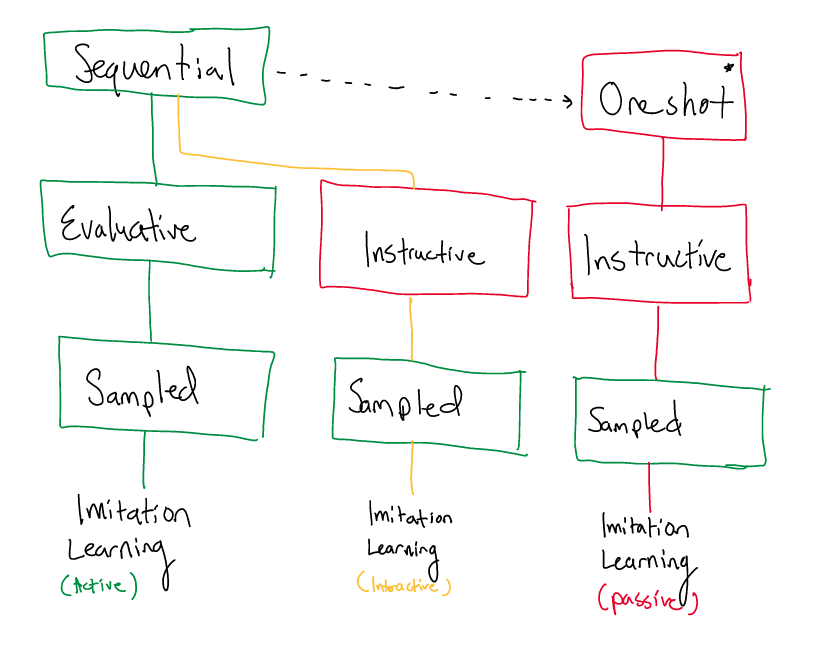
\includegraphics[width=4.5in]{class.png}
\caption{Imitation Learning vs. Learning Trajectory\cite{RL-circle}} 
\label{img:class}
\end{figure}

Imitation learning can be described using the same MDP we used for RL with some minor modifications. Similar to RL: $S$ is equal to the state, $A$ is equal to the action, $P$ is the transition dynamics, $P(s'|s,a)$ is equal to the probability of achieving $s'$ from state $s$ through action $a$ and $r$ is equal to the reward. We will now delve into the details of each part of the IL structure:

\begin{itemize}
    \item \textbf{Expert Demonstrations}
    \begin{equation}
        D^* = \{\zeta_n\}_{n=1}^N\sim \varepsilon|\pi^*
    \end{equation}
    Expert demonstrations are the new addition to our previous RL algorithms and are one of the centerpieces of IL. Expert demonstrations are sequences of states and actions that are sampled from the optimal policy. The learner has to find a policy that fits the trajectories sampled at all or most states without over-fitting to a single sample. This is difficult and is why there are many techniques to solve this problem. The trajectories are defined as follows: $\zeta=\{s_0, s_1,...s_T\}$ where $s_0 \rightarrow s_1$ is a transition between one state to another. $\zeta=\{s_0, a_0, s_1, a_1,...,a_{T-1},s_T\}$ is equal to the state-action steps in the sequence and explicitly states the action required to transition from one stat to the next. 
    
    Note that the expert demonstrations are often assumed to be optimal, but that is not always the case in practice. They may just provide a decent starting policy for the IL algorithm to interact with its environment, as was the case in \cite{baseballRL}.
    
    \item \textbf{Oracle}
    \begin{equation}
        \pi^*(a|s)
    \end{equation}
    
    The oracle knows $\pi^*$, the optimal policy for the system. It uses this policy to help the IL algorithm improve. The IL algorithm learns from the oracle by interacting with its environment, and getting feedback on if its actions were optimal or not. Through these interactions, the IL algorithm can improve its policy toward the optimal policy.
    
    \item \textbf{Dynamics}
    \begin{equation}
        \mathcal{T} = P(s'|s,a)
    \end{equation}
    The dynamics function for IL is the same as the one used for RL. It is the probability of getting to state $s'$ from state $s$ through action $a$. One thing to note in IL is that the dynamics function is not always given. An example of this in passive IL is the behaviour cloning  algorithm (also known as supervised learning), which does not assume a knowable dynamics function. We will delve further into this later on in the scribe notes.
    
    \item \textbf{Reward}
    \begin{equation}
        \mathcal{R} = R(s,a,s')
    \end{equation}
    Reward functions are also defined similarly to how we defined them in RL. Based on state $s$, doing action $a$ and iterating to the next state $s'$ a reward $r$ is generated. RL and IL both choose actions through policies and the policies can be chosen scholastically. However, as we have mentioned above, IL uses some form of expert/oracle feedback directly or in conjunction with RL to estimate the policy, and in the case of IRL, to also re-estimate the reward function.

\end{itemize}

\subsection{Imitation Learning: Types}

In Table~\ref{tab:type} below we outline the three major types of IL and how they differ with regards to state parameters and information exposure: 

\begin{table}[h]
\centering
\begin{tabular}{|c|c|c|c|}
\hline
\textbf{Parameter} & \textbf{Passive} & \textbf{Active} & \textbf{Interactive} \\ \hline
Demonstration $\mathcal{D}^*$     & yes        & yes       & optional       \\ \hline
Environment $\varepsilon$ & no         & yes       & yes            \\ \hline
Oracle $\pi^*$           & no         & no        & yes            \\ \hline
Dynamics $\mathcal{T}$             & no         & optional  & optional       \\ \hline
Reward $\mathcal{R}$               & no         & optional  & optional       \\ \hline



\end{tabular}
\caption{Imitation Learning Types}
\label{tab:type}
\end{table}

We will now delve a bit deeper into those definitions and explore what each type of IL described above entails:

\begin{itemize}
    \item \textbf{Passive}
    Passive reinforcement learning, also known as supervised learning or behavior cloning, uses only trajectory demonstrations provided by the expert to learn a policy. Policy optimization's sole purpose in these algorithms is to match the behavior of the expert (supervised data). This can be formulated as:
    \begin{equation}
    \arg\min_\theta\sum_{\tau=\{s_t,a_t\}_{t=1}^T} l(\pi_\theta(a|s_t), a_t)
    \end{equation}
    
    One thing to be wary of when using passive reinforcement learning algorithms is \textbf{covariate shift}, which is when error accumulates due to several successive states that were not seen in training. Since the agent has not seen these states before, it will likely not behave optimally, resulting in error at each state. In sequential settings like driving, this error can compound across several adjacent states and result in the agent failing.  
    
    \item \textbf{Active}
    For the active version of IL, we have access to the environment and the expert demonstrations. This means that the learner can train an initial policy using the expert demonstrations, and then use RL techniques to improve the policy by interacting with the environment. This allows the learner to identify differences between the demonstrations it received and the environment it acts in, and update its policy accordingly. It also allows the learner to improve upon its policy if the expert demonstrations were not optimal.
    
    In active IL, the learner also sometimes has access to the state transition dynamics and reward function of the environment. 
    
    \item \textbf{Interactive}
    In interactive IL, the learner can access feedback from an oracle that knows $\pi^*$, the optimal policy. This allows it to directly improve its policy after each non-optimal action that it takes. With the oracle, initial expert demonstrations are not necessary since oracle feedback can effectively provide those in hindsight. Note that this is not a good approach in environments where failures can be expensive (e.g. driving). The state transition dynamics and reward function are optional for these algorithms, but often are not needed due to the presence of the oracle.
    
\end{itemize}

\subsection{Inverse Reinforcement Learning: Overview}

A form of active IL is "Inverse Reinforcement Learning" (IRL). The idea behind IRL is that the reward function, which is usually elusive, can be learned in reverse through IRL then fed into RL to derive the optimal policy  $\pi$. IRL learns the optimal reward function from the expert, the learner, and the behaviors they both demonstrate. This type of reward function does well in generalizing the problem to different (but similar) environments and is a very powerful solution.

The outline of the architecture of Inverse Reinforcement Learning is shown in Figure \ref{img:irl}:

\begin{figure}[H]
\centering
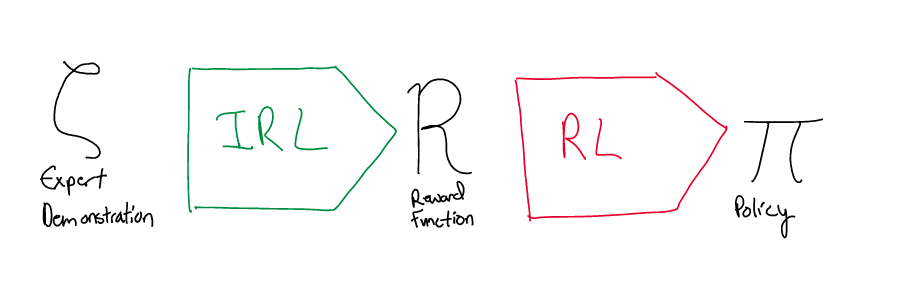
\includegraphics[width=4.5in]{irl.png}
\caption{Inverse Reinforcement Learning}
\label{img:irl}
\end{figure}

\subsection{Inverse Reinforcement Learning: Types}

\begin{itemize}
    \item \textbf{Finite State Space}
    In finite state space IRL we assume that the set of all possible states is finite, that the transition model is known, and that the complete policy is knowable for our learner. This is the simplest case and a great base to start with.
    
    \item \textbf{Large State Space}
    In large state space IRL we assume that the set of all possible states is very large or infinite, that the transition model is known, and that the complete policy is knowable for our learner. This will be a bit more challenging and will require some derivation to approximate.
    
    \item \textbf{Sampled Trajectories}
    This will be covered in the following lecture, and will relax more assumptions that will allow the IRL algorithm to become even more generalizable.
\end{itemize}

\subsection{Inverse Reinforcement Learning: Finite Spaces} 
In lecture, we discussed the parking lot trajectory planning problem as an example of a finite space IRL problem. In this case, we discretized the parking lot into a grid area, labelled each grid with some features, and then trained a reward function using this information and expert demonstrations. This reward function allowed us to classify the rewards of different parts of a scene, which we could use to plan trajectories in different scenes. Note that these scenes still need to be similar to the original unless we are given more demonstrations related to the new scenes. For example, the parking lot trajectory demonstrations will not train a good reward function for generating trajectories on hikes in wooded areas. This framework is depicted in Figure \ref{img:irl_parking_lot}.

When solving finite space inverse reinforcement learning problems, we assume that:
\begin{itemize}
    \item state space is finite
    \item transition model is known
    \item optimal policy is known
\end{itemize}

These problems can be represented with the following optimization problem:

$$
\max\limits_R \Large{ \sum\limits_s Q^{\pi}(s, a^*) - \max\limits_{a \neq a^*} Q^{\pi} (s,a) \Large}
$$

This means we want to find a Q function that maximizes the improvement of the optimal policy over the second best action at every state. In other words, we are trying to find the reward function that makes the given policy optimal by the largest margin. One thing to be wary of is that, if left unconstrained, this optimization will result in massive positive or negative rewards at different states. To fix this, you can add a penalty term on the sum of the absolute values of the rewards (also known as the L1 norm):

$$
\max\limits_R \Large{ \sum\limits_s Q^{\pi}(s, a^*) - \max\limits_{a \neq a^*} Q^{\pi} (s,a) \Large}
- \lambda ||R||_1
$$

This problem can be solved with a linear program. To do so, you first need to use the matrix form of the Q table:

$$
Q^{\pi}(s,a) = R(s) + \gamma \sum\limits_{s'} p(s' | s,a) V^{\pi}(s') \forall s,a
$$
$$
\textbf{Q}^{\pi}(a) = (\textbf{R} + \gamma \textbf{P}_a \textbf{V}^{\pi})
$$

We can do the same thing with the Value Function $V^{\pi}(s)$:

$$
V^{\pi}(s) = R(s) + \gamma \sum\limits_{s'} p(s' | s,a = \pi(s)) V^{\pi}(s') \forall s
$$
$$
\textbf{V}^{\pi} = (\textbf{I} - \gamma \textbf{P}_a)^{-1} \textbf{R}
$$

This allows us to write the objective function as:
$$
\textbf{Q}^{\pi}(a^*) - \textbf{Q}^{\pi}(a)
$$
$$
= (\textbf{R} + \gamma \textbf{P}_{a^*} \textbf{V}^{\pi})- (\textbf{R} + \gamma \textbf{P}_a \textbf{V}^{\pi})
$$
$$
= \gamma (\textbf{P}_{a^*} - \textbf{P}_{a}) (\textbf{I} - \gamma \textbf{P}_{a^*})^{-1} \textbf{R} 
$$

Before we can write the objective function in linear form, there is one more constraint we need to add. This is that the future payoff for the optimal action is greater than the future payoff for any other action. We can write this in matrix form like so:

$$
\textbf{P}_{a^*} \textbf{V}_{\pi} \geq \textbf{P}_a\textbf{V}_{\pi}
$$

Plugging in the expression we derived for $\textbf{V}_{\pi}(s)$:

$$
\textbf{P}_{a^*} (\textbf{I} - \gamma \textbf{P}_{a^*})^{-1} \textbf{R} \geq \textbf{P}_a (\textbf{I} - \gamma \textbf{P}_{a^*})^{-1} \textbf{R}
$$

Now we can write out the full description of the linear program:

$$
\hat{R} = \text{arg}\max\limits_{R} \Big( \sum\limits_s \min_a \big\{ \gamma (\textbf{P}_{a^*} - \textbf{P}_{a}) (\textbf{I} - \gamma \textbf{P}_{a^*})^{-1} \textbf{R} \big\} \Big) - \lambda ||R||_1
$$
$$
\text{s.t.} \quad (\textbf{P}_{a^*} - \textbf{P}_{a}) (\textbf{I} - \gamma \textbf{P}_{a^*})^{-1} \textbf{R} \geq 0
$$
$$
|R(s)| \leq R_{max} \forall s \in S
$$


\begin{figure}[H]
\centering
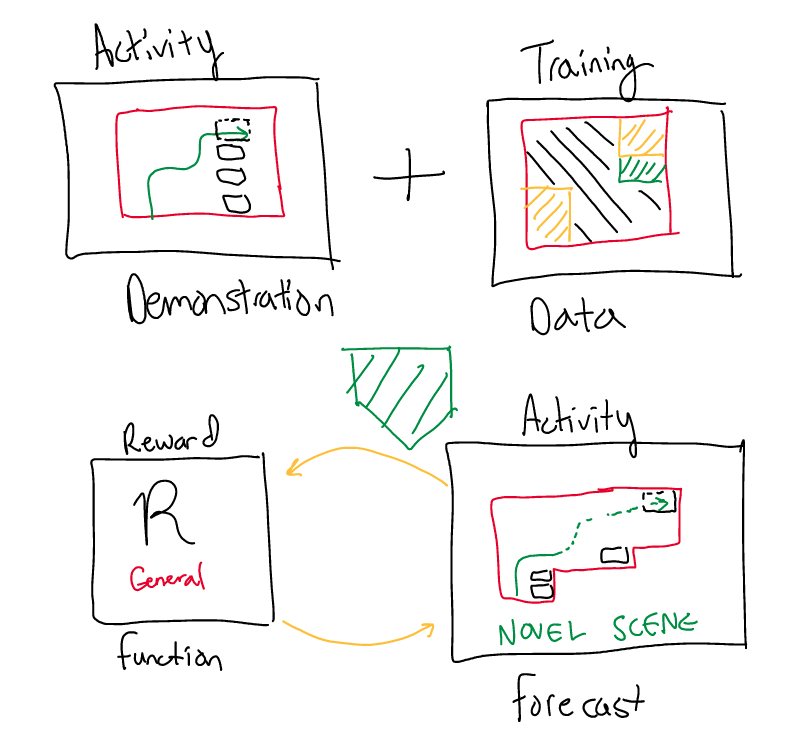
\includegraphics[width=4.5in]{parking.png}
\caption{Finite Space IRL Parking Lot Example \cite{activityForecasting}} 
\label{img:irl_parking_lot}
\end{figure}


% \nocite{*}
\bibliography{refs} 
\bibliographystyle{abbrv}



%\section{Appendix}
%This section provides any relevant background material that was not covered in the lectures, but was found to be useful for understanding the material. 
%For example, derivations, theory underlying techniques employed, etc. 

%Additionally, this section can summarizes applications or extensions of these techniques found in the literature. 

\end{document} % Done!


